\documentclass[12pt,french]{book}
\input preambule_2013
\input philippe2013_activites
\pagestyle{empty}


\begin{document}

\TitreActivite{vi.1}{Une fonction affine\\ en physique}

\begin{minipage}{0.3\linewidth}
    \begin{center}
        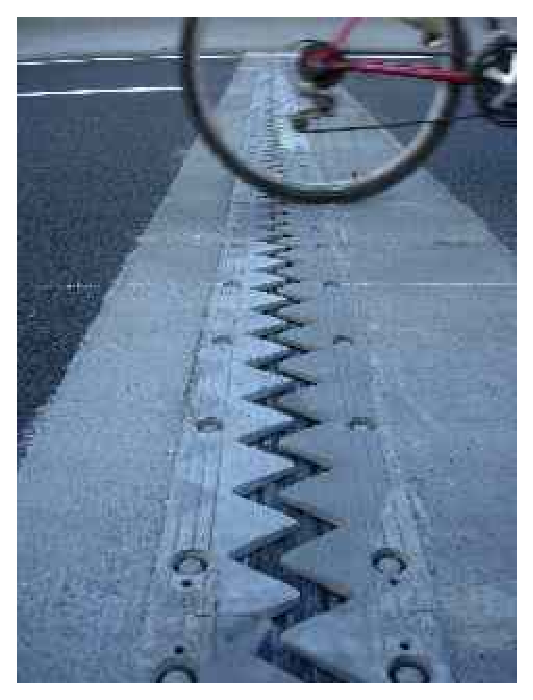
\includegraphics[scale=0.35]{joint_dilatation_pont.eps}
    \end{center}
\end{minipage}
\begin{minipage}{0.69\linewidth}
    La dilatation linéaire est un phénomène physique qui se traduit par une augmentation de la longueur d'une barre ou d'un fil lorsque la température augmente.\par\smallskip
    Ce phénomène, bien connus des physiciens, peut causer des dégâts sur des constructions, notamment à structure métallique, comme les rails de chemin de fer, ou de ponts.
\end{minipage}\medskip

On considère une barre de longueur initiale égale à $L_i$ (en mètre) à la température initiale de $t_i\degres$\bsc{c}. Si la température augmente pour atteindre $T\degres$\bsc{c}, alors, par phénomène de dilatation linéaire, la barre s'allonge et atteint une longueur $L(T)$ (en mètre) définie par :
\[L(T) = L_i \times \big(1 + \lambda (T - t_i)\big) \quad \text{(la lettre grecque $\lambda$ se lit << lambda >>)}.\]
Le nombre $\lambda$ est appelé c{\oe}fficient de dilatation linéaire et dépend du matériau.\bigskip

\begin{enumerate}
    \item Montrer que $L$ est une fonction affine dépendant de la température $T$.
    \item \textbf{Quelques exemples avec de l'acier :}\par
    Pour l'acier, le c{\oe}fficient de dilatation est égal à $\lambda = 12 \times 10^{-6}$.
    \begin{enumerate}
        \item \'Ecrire $\lambda$ sous forme décimale.
        \item En hiver, à une température de $-20\degres$\bsc{c}, un rail en acier d'une ligne de chemin de fer mesure $30~m$ de long. Un été, la température atteint $40\degres$\bsc{c}.\par
        On a donc $L_i = 30$, $t_i = -20$ et $T = 40$.\par
        Calculer la longueur du rail en été. À combien est égale l'augmentation de la longueur du rail en $cm$ ?
        \item Lorsqu'il fait $10\degres$\bsc{c} à Paris, la tour Eiffel mesure $327$ mètres.\par Un été, la température atteint $35\degres$\bsc{c}.\par
        De combien de centimètres la tour Eiffel a grandi cet été là ?
        \item Le pont de Normandie a une longueur de $\np{1420}~m$.
        \begin{center}
            \includegraphics[scale=0.75]{Pont_Normandie.eps}
        \end{center}
        Si l'on suppose que sa structure en acier est faite d'une seule pièce, quel serait l'allongement total de ce pont si la température augmentait de $50\degres$\bsc{c} ?\par
        Quel problème poserait ce résultat ?
    \end{enumerate}
\end{enumerate}


\end{document}
